\documentclass[]{article}
\newcommand{\FileDepth}{../..}
\input{\FileDepth/Formats/AssignmentBasics.tex}
\usepackage{cancel}%This is special for Activities 4 and 5.
%opening
\newcommand{\SecType}{X}
\newcommand{\Week}{X}
\title{Steady Block on a Sliding Ramp}
\author{Benjamin Bauml}
\date{Spring 2024}
\pagestyle{fancy}
\rhead{PH 221}
\chead{Spring 2024}
\lhead{Week \Week}

% For Assignment, leave Purpose as 1. For Worksheet, set to 2. For Student Solution, set to 3. For Teacher Solution, set to 4.
% If you want keep the pieces from being called manually, set DefOnly to 0.
\newcommand{\Purpose}{4}
\newcommand{\DefOnly}{1}

% Version 2024-04-27
% Changes
% 2024-02-21 Added xstring package to enable smooth implementation of new \ModePage command.
% 2024-04-27 Set up to split activities and formatting aspects into separate files. Removed dependence on xcomment. Added an automatic counter to number the activities in a problem set.
\usepackage{tcolorbox}
\usepackage{xstring}
% You will want the following four lines in your document (the last two uncommented):
% For Assignment, leave Purpose as 1. For Worksheet, set to 2. For Student Solution, set to 3. For Teacher Solution, set to 4.
% If you want keep the pieces from being called manually, set DefOnly to 0.
%\newcommand{\Purpose}{4}
%\newcommand{\DefOnly}{1}
\newcommand{\Exclusion}{0}
\newcommand{\PageTurn}{0}
\newcommand{\GrayProb}{0}
\newcommand{\Tipsy}{0}

% Assignment
\if\Purpose1
\renewcommand{\Exclusion}{1}
\fi
% Worksheet
\if\Purpose2
\renewcommand{\Exclusion}{1}
\renewcommand{\PageTurn}{1}
\fi
% Student Solution
\if\Purpose3
\renewcommand{\PageTurn}{1}
\renewcommand{\GrayProb}{1}
\fi
% Teaching Copy
\if\Purpose4
\renewcommand{\PageTurn}{1}
\renewcommand{\GrayProb}{1}
\renewcommand{\Tipsy}{1}
\fi

\def \NewQ {0}
\def \PForce {0}
\newcommand{\MaybePage}[1]{
	\def \PForce {#1}
	\if\PForce1
	\newpage
	\else
	\if\NewQ0
	\gdef \NewQ {\PageTurn}
	\else
	\newpage
	\fi
	\fi
}

\newcommand{\ModePage}[1]{
	\IfSubStr{#1}{\Purpose}{\newpage}{}
}

\newcounter{ActNumber}
\setcounter{ActNumber}{0}

\newcommand{\Problem}[4][0]{%The first argument is optional, and if it is set to 1, the \newpage will be forced. The second argument is the name of the activity, the third is the command the activity is stored as, and the fourth is the actual problem statement.
\newcommand{#3}{
\MaybePage{#1}
\addtocounter{ActNumber}{1}
\section*{\SecType\Week-\theActNumber: #2}
\if\GrayProb1
\begin{tcolorbox}[colback=lightgray,colframe=lightgray,sharp corners,boxsep=1pt,left=0pt,right=0pt,top=0pt,bottom=0pt,after skip=2pt]
\else
\begin{tcolorbox}[colback=white,colframe=white,sharp corners,boxsep=1pt,left=0pt,right=0pt,top=0pt,bottom=0pt,after skip=2pt]
\fi
#4
\end{tcolorbox}\noindent
}
\if\DefOnly0
\else
#3
\fi
}
	
\newcommand{\ProblemSub}[3][0]{%The first argument is optional, and if a string of numbers is entered into it, it will force a \newpage in any \Purpose that shows up in the string. For example, "13" would lead to the newpage being forced in modes 1 and 3. The second is the command the activity is stored as, and the third is the actual problem statement.
\newcommand{#2}{
\ModePage{#1}
\if\GrayProb1
\begin{tcolorbox}[colback=lightgray,colframe=lightgray,sharp corners,boxsep=1pt,left=0pt,right=0pt,top=0pt,bottom=0pt,after skip=2pt]
\else
\begin{tcolorbox}[colback=white,colframe=white,sharp corners,boxsep=1pt,left=0pt,right=0pt,top=0pt,bottom=0pt,after skip=2pt]
\fi
#3
\end{tcolorbox}\noindent
}
\if\DefOnly0
\else
#2
\fi
}
		
\newcommand{\Solution}[2]{%The first argument is the command the solution is stored as, and the second is the actual solution.
\newcommand{#1}{
\if\Exclusion0
#2
\fi
}
\if\DefOnly0
\else
#1
\fi
}
		
\newcommand{\ProblemFig}[2]{%The first argument is the command the figure is stored as, and the second is the actual figure.
\newcommand{#1}{
\begin{figure}[h]
#2
\end{figure}
}
\if\DefOnly0
\else
#1
\fi
}
		
\newcommand{\TeachingTips}[1]{
\if\Tipsy1
\begin{tcolorbox}[colback=lightgray,colframe=black]
#1
\end{tcolorbox}
\fi
}

\newcommand{\FBDaxes}[4][2]{
	\begin{scope}[shift={(#2)},rotate=#3]
		% x-axis
		\draw[thick,->] (-#1,0) -- (#1,0);
		\node[anchor=west] at (#1,0) {$x$};
		% y-axis
		\draw[thick,->] (0,-#1) -- (0,#1);
		\node[anchor=south] at (0,#1) {$y$};
		\coordinate (#4) at (0,0);
	\end{scope}
}
\newcommand{\FBDvectorMA}[4]{
	\begin{scope}[shift={(#1)}]
		\coordinate (#4tip) at ({#2*cos(#3)},{#2*sin(#3)});
		\draw[ultra thick,blue,->] (#1) -- (#4tip);
	\end{scope}
}
\newcommand{\FBDvectorXY}[3]{
	\begin{scope}[shift={(#1)}]
		\coordinate (#3tip) at (#2);
		\draw[ultra thick,blue,->] (0,0) -- (#3tip);
	\end{scope}
}
\newcommand{\FBDdot}[1]{
	\filldraw[black] (#1) circle (3pt);
}
\newcommand{\FBDbox}[5][1]{
	\begin{scope}[shift={(#2)},rotate=#3]
		\filldraw[color=black,fill=white,thick] ({-#1/2},{#1/2}) -- ({-#1/2},{-#1/2}) -- ({#1/2},{-#1/2}) -- ({#1/2},{#1/2}) -- cycle;
		% Left side coordinates
		\coordinate (#4ltq) at ({-#1/2},{#1/4});
		\coordinate (#4lcent) at ({-#1/2},0);
		\coordinate (#4lbq) at ({-#1/2},{-#1/4});
		% right side coordinates
		\coordinate (#4rtq) at ({#1/2},{#1/4});
		\coordinate (#4rcent) at ({#1/2},0);
		\coordinate (#4rbq) at ({#1/2},{-#1/4});
		% top coordinates
		\coordinate (#4tlq) at ({-#1/4},{#1/2});
		\coordinate (#4tcent) at (0,{#1/2});
		\coordinate (#4trq) at ({#1/4},{#1/2});
		% bottom coordinates
		\coordinate (#4blq) at ({-#1/4},{-#1/2});
		\coordinate (#4bcent) at (0,{-#1/2});
		\coordinate (#4brq) at ({#1/4},{-#1/2});
		% corners
		\coordinate (#4tl) at ({-#1/2},{#1/2});
		\coordinate (#4tr) at ({#1/2},{#1/2});
		\coordinate (#4bl) at ({-#1/2},{-#1/2});
		\coordinate (#4br) at ({#1/2},{-#1/2});
		\node at (0,0) {#5};
	\end{scope}
}

\begin{document}
\maketitle
\begin{center}
	This material is borrowed/adapted from PH 201 Tutorial 5 for Fall 2020 and Mastering Physics.
\end{center}

\Problem{Steady Block on a Sliding Ramp}{\SteadyBlock}{
A block of mass $m$ sits upon a frictionless ramp (inclined at angle $\theta$) that is being pushed to the right. What must the acceleration of the ramp be to prevent the block from sliding down the surface?
}
\ProblemFig{\SteadyBlockFig}{
\centering
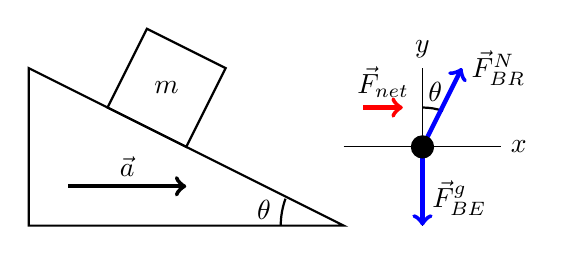
\begin{tikzpicture}
	\draw[thick] (0,0) -- (4,0) -- (0,2) -- cycle;
	\draw[thick] (3.2,0) arc (180:160:1);
	\node[anchor=east] at (3.2,0.2) {$\theta$};
	\draw[thick] (1,1.5) -- (2,1) -- (2.5,2) -- (1.5,2.5) -- cycle;
	\node at (1.75,1.75) {$m$};
	\draw[ultra thick,->] (0.5,0.5) -- (2,0.5);
	\node[anchor=south] at (1.25,0.5) {$\vec{a}$};
	\if\GrayProb1
	\draw (4,1) -- (6,1);
	\node[anchor=west] at (6,1) {$x$};
	\draw (5,0) -- (5,2);
	\node[anchor=south] at (5,2) {$y$};
	\draw[thick] (5,1.5) arc (90:71:0.8);
	\node[anchor=west] at (4.95,1.7) {$\theta$};
	\draw[ultra thick,blue,->] (5,1) -- (5.5,2);
	\node[anchor=west] at (5.5,2) {$\vec{F}^{N}_{BR}$};
	\draw[ultra thick,blue,->] (5,1) -- (5,0);
	\node[anchor=south west] at (5,0) {$\vec{F}^{g}_{BE}$};
	\filldraw[black] (5,1) circle (4pt);
	\draw[ultra thick,red,->] (4.25,1.5) -- (4.75,1.5);
	\node[anchor=south] at (4.5,1.5) {$\vec{F}_{net}$};
	\fi
\end{tikzpicture}
}
\Solution{\SteadyBlockSol}{

If the block is not sliding down the surface of the ramp, then it is moving with it, so the acceleration of the block must be the same as that of the ramp, which points directly to the right. Since we know the direction of acceleration, it will be advantageous to set up our coordinate system with one of the axes along that direction. This differs from several other ramp problems, where a tilted coordinate system is advantageous due to there being fewer vectors to break into components.

If acceleration is along the $x$-axis, as depicted above, we need the two forces (the force on the block normal to the surface of the ramp and the force of gravity on the block) to cancel in the $y$-direction. As such,
\[
0=F^{N}_{BR,y}+F^{g}_{BE,y}=F^{N}_{BR}\cos\theta-mg \implies F^{N}_{BR}\cos\theta=mg \implies F^{N}_{BR}=\frac{mg}{\cos\theta}.
\]
Meanwhile, in the $x$-direction, we only have the $x$-component of the normal force, so
\[
F_{net,x} = F^{N}_{BR,x} = F^{N}_{BR}\sin\theta = mg\frac{\sin\theta}{\cos\theta} = mg\tan\theta.
\]
Since $F_{net,x}=ma_{x}=ma$, we can cancel out the mass to obtain
\[
a = g\tan\theta.
\]
In the special case of a flat ramp, which we expect does not need to move to keep the box from sliding, we have $\theta=0$, and thus $\tan\theta=0$, so our equation indeed gives us $a=0$. Alternatively, if the ramp is vertical, then we cannot keep the block from sliding, as there is nothing beneath it to hold it up. This is the $\theta\to90^{\circ}$ case, and that gives us $a=g\tan\theta\to\infty$, since there is not a finite acceleration sufficient to hold up the block.
}
\end{document}